\autsection{Defining life}{Agge Winther, Fruzsina Bacso} 

One of the main objectives, if not the main objective, on this mission is to search for life. This is after all a life finding mission and therefore the instrument suite on-board needs to be focused on finding life. The mission is going to look for life in the ice and mostly in the water below the ice, where there is a high expectancy to find some sort of life or life harbouring conditions.

Life can be found in many forms and stages of evolution, and it can therefore be very difficult to detect, because we do not know exactly what the penetrator should look for. Before looking into what we should look for on Europa, a set of guide rules needs to be put in place, defining what life forms are already known from earth. It would be ideal to set up a precise yardstick for life, a list of things needed to say that life will exist, but this is not possible. What is possible is to look at what is present on Earth and applying this to alien life forms.

Most living organisms as we know from Earth have some properties in common, though non-living matter show some of them, only living organisms show all of them\cite{WhatIsLife}. The 7 properties are:
\begin{enumerate}
  \item Organization
  \item Metabolism
  \item Homeostasis
  \item Growth
  \item Reproduction
  \item Response
  \item Evolution
\end{enumerate}
Beginning at number one "Organization", to have life, structure is needed, and by taking unorganized matter and organizing it, is a sign of life. Living organisms a made up of one or more cells which in them self are highly organized, and able to produce complex chemical processes from an unorganized energy source. For bigger multi-cell organisms, organization is important, since individual cells are assigned different specific jobs to create a bigger and more complex organism.

Metabolism is the life sustaining chemical transformations happening within cells and living organisms, and is the sum of all chemical reactions happening in a living organism. This chemical conversion can be divided into two subcategories, catabolism and anabolism. Catabolism is the process of breaking down organic matter into energy, with anabolism being the reverse process, building up complex molecules such as protein from simple molecules. This type of process uses energy. One of the most important metabolisms, is the citric acid cycle (Krebs cycle), it is believed to be one of the early established components for cellular metabolism.

Most living cells and organisms have a working area where they are able to sustain life; humans need to stay a cool 37 degrees to function normally. The ability to maintain a stable internal environment, even with a varying external environment is called homeostasis. This type of process is mostly found in more complex organisms, like smaller animals. Microorganisms usually depend on their surroundings to create a stable living environment.

The fourth properties is growth, this begins at a cellular level and is linked to the organization of the cells in defined structures. It depends on the anabolism to crate proteins and amino acids for DNA. Without growth more complex molecules and organisms would not exist.

Reproduction is also important for sustained life, looking at single cell organism like bacteria, which is able to reproduce by simply splitting in two. Reproduction can also take place with two parent organisms creating a new cell from a combination of both their genetic information.

Organisms need to respond to actions from their environment to be able to survive. That is way many plants turn towards the sun, and bacteria cluster together around a nutrient rich area. When provoking a living organism, heating it, burning it, a response should be detected. It does not need to be movement, it could also be creating a toxin release or other chemical, helping it defend or survive from an unknown threat.

Lastly it needs to evolve, their genetics needs to adapt to changes, making it stronger and able to survive. Here natural selection is involved, where traits which make it easier to survive are carried through, by the death of the weaker organism that did not evolve. This is of cause a very slow process, but might be the key to discovering life on other planets, due to its adaptability.

These 7 properties of life are all found in living organisms on earth, this does not mean that the yard stick for life is defined perfectly, it is not! It is still hard to define life exact, and this only guides us some of the way. An example of where this does not hold true is for a mule, it is very much alive but is not able to reproduce\cite{Mule}.

The properties can give an idea of what to look for when doing analysis of samples from Europa, because some of the processes create by-products that could be detected. One of the most well known processes with this ability is photosynthesis, taking $CO_2$ and energy to create sugar and oxygen. It takes the suns energy and harvests it into chemical energy which can be used as fuel for the organisms. This type of process is very unlikely to take place in the ice or water of Europa, since the sun is 780 million kilometres away, and no light will get through the ice and down in the ocean. In general life needs to be rethought for the Europan environment.

A good place to start the search for life is at the building block level, and looking for process that needs a source of energy, most likely heat, and some chemicals/nutrients, to create sustained life. This type of process is called abiogenesis\cite{Abiogenesis} and is the natural process of living organisms arising from non living matter. The search could therefore go into look for simple non living matter such as simple organic compounds. This will narrow the search down to looking for molecules containing carbon, like in simple carbohydrates, this is of cause just one basic assumption for life, the other obvious one is the energy. No sunlight is reaching the ocean so energy must be created differently, by gravity or thermal activity in the rock core, this will be investigates further in the next chapters.

If the energy is there and some simple organic compounds can be found, life might be able to exist. The search therefore need to be increased to look for more complex molecules, here the organization property comes to play.  Now the search for proteins, and single celled organism, like bacteria would be possible living organisms.

This would go on, into bacteria colonies and even more complex organisms, but the conclusion is that we need some simple organic building blocks and energy to create some sort of life here on Earth (important distinction). Making a more generalized plan for what life is some other aspects needs to be taking into account by looking even further back to the origin of life.

\subsection{Hypotheses about the origin of life on Earth}

This is one of the difficult ones, because sciences do not know for sure how life came to be, but some important hypotheses have been made around where and how life on Earth originated from.

Life on Earth started some 3.5 billion years ago, the evidence for this is found in rock structures around the world, as small fossils of microbes. One place this is still evident today is in stromatolites which are produced by microbes by photosynthesis. They form a layer of microbial film, trapping mud under it, creating lay upon layer of mud and microbes, some dating back to 3.5 billion years ago.

The earliest signs of life are found on land, the main hypothesis to where life originates from is in the oceans, more specific the thermal vents on the deep sea ocean floor. The conditions found around these black smokers are ideal for an abiogenesis, due to the chemicals present and the energy in form of heat from the vents. DNA sequencing also suggest that some of the early life was microorganisms living in an aquatic high temperature environment.

As talked about in the previous chapter, life is complex, even on a microbe/bacteria level. These complex cells did not just show up, they evolved through small steps and natural selection. Hypotheses to how these more complex multi-celled organisms came to be can be split up in to 5 steps:
\begin{enumerate}
  \item In the beginning of Earth life, the atmosphere consisted of nitrogen, hydrogen, ammonia, water vapor and methane. This was able to combine in to simple organic matter, such as nucleotides found in RNA and DNA.
  \item The foundation was now set, and next came self replication molecules. These molecules are chains of nucleotides, and are able to replicate them self by some sort of RNA self-replicator process. With self-replicating came also natural selection, not all replications went well, and therefore some survive better than others. This process continued creating more and more stable and efficient replication processes.
  \item These replicating cells then got enclosed in a cell membrane, protection the self-replication molecules, these cells had a great advantages over the non enclosed cells, due to the protection of the internal environment from the outside environment.
  \item All of this was based on RNA-processes, but when some cells evolved to use DNA, things changed. Now instead of RNA doing the whole replication process, DNA became the genetic material, it is also more stable then RNA, proteins became responsible for metabolism inside the cell and RNA now only did the part of carrying information from the DNA to the protein building areas of the cell. This new replication process is seen in \ref{fig:RNAtoDNA}.
  \item Instead of the cells always splitting up after self replication, some stated to form more complex multi-celled organisms, the beginning of multi-cellular organisms.
\end{enumerate}
\begin{figure}[htb]
  \centering
  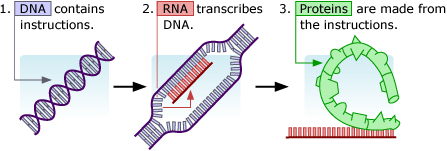
\includegraphics[width=\textwidth]{figures/Life/dnarnaprotein}
  \caption{The RNA is now the message carrier, and the DNA became the genetic material}
  \label{fig:RNAtoDNA}
\end{figure}
This was a short investigation into how life on earth could have evolved. Some of the hypotheses are still investigated and some gaps are still to be filled. An example of this is how RNA and proteins where created, because nucleic acids for DNA and RNA productions depend on proteins, but to build proteins nucleic acids are needed. The solution to this problem was first recently discovered, where the knowledge on RNA was expanded, and is was discovered that RNA is able to both store and copy itself concluding that nucleic acids came first \cite{UndestandingEvolution}.

Many of these processes are dependent on energy from the sun, and it was after the first stromatolites and their photosynthesis the atmosphere started changing and became more oxygen rich. This will have worked as a toxic gas on some anaerobic cells, making aerobic cells more common on land. This just shows how many factors play a role on how life originated and further evolved, killing the first evidence of life as other life forms evolved.

From all of this a conclusion can be drawn in what might be expected to be found on Europa, a uplifting clue is found in the black smokers on Earth, which could be found on the bottom of Europa. But from what we see on earth, the most likely life forms are bacteria, or simple multi-cellular life forms, and what we need to look for includes, simple organic compounds, such as carbohydrates, enzymes, lipids fatty acids, nucleic acids, proteins, peptides, amino acids are some of the important compounds which could indicate life or a habitat for life.

Another way to investigate life, is to look at the environment it is created from/in, and if life did exists we might see reminisce of life. The next two chapters look into the life harboring conditions and possible clues to look for from extinct life forms.

\subsection{Life harboring conditions and planetary habitability}

This chapter will look into the condition need for life to evolve on a planet, and since life beyond Earth is unknown, the theories on planetary habitability are built on what is known from Earth.

Planetary habitability, is a measure of a planet's ability to harbour life in a habitable environment\cite{PlanetaryHabitability}, this does not mean that life exists on the planet in question, but just that the conditions are right for life to develop, or to be transferred from another planet.

Some of the requirement for life has already been discussed previously, but show up again in this chapter. One of them is energy, there need to be some sort of energy present, apart from that many other geophysical and astrophysical criteria must be just right, for a planet, to be habitable. Looking at one of NASA's guide rules for life is "extend regions of liquid water\cite{NasaWater}"  since this is a great place for organic matter to form from, and here energy can come from either the sun in the top ocean layers, or for example black smokers on the bottom.

Habitability is not only dependent on the planets environment, atmosphere and so on, but also other externals needs to be considered; here we need to look at the astrophysical properties such as orbit and placement compared to the sun. In all there are many aspects to take in to account and like the chapter about "Defining life" some properties for habitability of a planet can be made:
\begin{enumerate}
  \item Mass
  \item Orbit and rotation
  \item Geochemistry
  \item Microenvironments and extremophiles
\end{enumerate}
The mass of a planet is important to sustaining an atmosphere; this is not a problem on Europa since the life is not expected to be found in its thin atmosphere. With smaller planets the energy left over from creation is lost faster making the planet geologically dead, this is a problem, since life is so dependent on an energy source. In the case of Europa the mass is very little compared to Earth which might point to a geological dead planet, and the energy must therefore come from the ice or the gravitational pull of Jupiter. But this does not always hold true, look at Jupiter's other moon Io, is geological active, and even with its little mass. This activity comes from the gravity pull from Jupiter.

In the orbit stability is key; a stable orbit gives stability to the environment on the planet. The speed of rotation and how elliptic the orbit is, influences the temperatures on the planet, here stable temperatures are favourable, so half the planet is not frozen half the year and boiled the next half year. Looking at Europa the problem is not that impotent, since if life is found, it is located in the water protected by the sounding ice.

The geochemistry tells if the fundamental building blocks are present to create the "food" for living organisms. The four important elements from know from Earth are nitrogen, hydrogen, carbon and oxygen. It was already discussed in the chapter about life origin why these are important.  It is hard to tell if these are present in the ocean on Europa, a NASA study describe the "Why look at Europa" describes how hydrogen and oxygen might be present in just the right quantities.

When looking at a new planet maybe only a small part of it is habitable, comparing with Earth 3.5 billion years ago, life was not as abundant as it is now. Therefore a small sample from Earth would not have shown any sign of life, even if there was in some extreme place such as at the black smokers on the ocean floor. On Earth organisms know as extremophiles live in these very niche environments with conditions not suitable for "normal" life, there can be temperatures above 100 degrees Celsius, or very acidic/alkaline conditions. This expands the possibility of finding life in more extreme environments such as on Europa.

All of this can be summarized in a list of factors; the list was originally made for reproducing and survival of Earth microbes on Mars. The list has been modified to match an environment with no atmosphere\cite{WaterMars}.
\begin{itemize}
  \item Water availability and activity
  \begin{itemize}
    \item Activity of liquid water
    \item Past/further liquid (ice)
    \item Salinity and pH
  \end{itemize}
  \begin{itemize}
    \item  Chemical environment
    \begin{itemize}
      \item Nutrients
      \begin{itemize}
        \item C, H, N, O, P, S, essential metals and micronutrients
        \item Fixed nitrogen
        \item Their availability/mineralogy
      \end{itemize}
      \item Toxin
      \begin{itemize}
        \item Heavy metals (Zn, Ni, Cu, Cr, As, Cd, etc.)
        \item Globally distributed oxidizing soils
      \end{itemize}
    \end{itemize}
  \end{itemize}
  \begin{itemize}
    \item  Energy for metabolisms
    \begin{itemize}
      \item Solar/Radiation
      \item Geochemical
      \begin{itemize}
        \item Oxidants
        \item Reductants
        \item Redox processes
      \end{itemize}
    \end{itemize}
  \end{itemize}
  \begin{itemize}
    \item Physical condition
    \begin{itemize}
      \item Temperature
      \item Small temperature fluctuations
      \item High $CO_2$ concentrations
      \item Water/ice flow
    \end{itemize}
  \end{itemize}
\end{itemize}
This list gives a good yard stick for determining if the planet is habitable, when Earth life forms are considered. Of cause life could be of a whole other unknown type which today's technology cannot detect and this will give problems which is left out of this discussion.

\subsection{Extinct life}

Due to the small size of Europa, it might be geologically dead, but life might have thrived when the planet still had left over energy from its creation. Therefore it would be an idea to look for signs of extinct life, as we also see from Earth, previous life literally fuels today's world.

When look for extinct life the search for distinct bio-makers/features that would indicate that life once thrived here. The things too look for will be leftovers from living organisms, this includes reduced carbon and nitrogen ($CO_3$(2-), $NO_3-$, $NO_2-$, $SO_4$(-2), also some important metals would be of interest Mg, Mn and Fe. But some of these compounds might not come from extinct life and it is therefore important to distinguish between biologically and not biologically produced compounds. An example of this is seen in the way $N_2$ is deposited, with no biological processes the $N_2$ would become $NO_3-$ and $NO_2-$, but if this is used on a biological process it would form $N_2$O or $N_2$ as a gas  (dependent on pressure)\cite{BiomarkersMars}.

From earth we see the extinct life in great quantizes such as oil and natural gas, produced by decomposing plants and animal matter under high heat and pressure. Natural gas is mainly made up of methane which would be a good marker for primordial life. Also oils floating on the water would indicate extinct life.

Through the last few chapters discussions about what life is and some of the signs to look out for have been investigated. Some of the findings have been applied to Europa and how it might fit the criteria as a life harbouring moon. In the last chapter a discussion about why Europa could be the place to go, for finding alien life in our solar system.

\subsection{Why look at Europa}

One of the most important properties of Europa is the liquid water found under the ice, which is key to life according to NASA, the more questionable, but just as important, is the energy need to create and sustain life. As discussed due to the small mass of Europa it might not be geologically active, if this is the case then a new NASA study carried out by JPL\cite{EuropasOceanLife} show that even without volcanic activity such as hydrothermal vents/black smokers, the balance of chemical energy might be there to support life. The study is based on methods know from Earth, and look at how energy and nutrients are carried around Earth's oceans. But most importantly how the production of hydrogen and oxygen will take place without volcanic activity, one of the methods fro creating oxygen is serpentinization, where water reacts with freshly exposed rock (cracks form when cooling or water movement) to produce hydrogen.

The other part of the study looks in to the production of oxidants and oxygen, here the radiation from Jupiter splits ice/water on the surface, which cycles into the ice and down to the ocean. Scientist does believe that compounds from the top ice slowly cycles through the icy surface. If the amount of oxidants and hydrogen produced Europa is balanced just right, it might have just the right conditions to sustain life.

It is already know that Io has volcanic activity due to the Jupiter's gravity push and pull on the rocky moon. This could indicate volcanic activity on Europa, giving even better conditions for life, due to the energy volcanic activity would bring. If Europa is geologically active there is a good chance of finding black smokers on the seafloor, this is one very important niche environment where life would thrive on the energy source and nutrients the black smokers produce.

Europa therefore seems like a perfect place to look for life and is also classified as a class III habitat. A planet in class III has liquid water of some sort trapped in or by ice, but since the water is enclosed the nutrient might be found in too small concentration to contain living organisms. This is the main problem with class III planet/moon, the lack of ingredients for life in one location due to the large water body and therefore lack of an incubator for life with the right amount of nutrients.

A illustration of all the possible methods for life to form is showed in \ref{fig:EuropaFromSurfaceToRockcore}, here radiation, ice cycle and volcanic activity would lead to a possible habitat for life in the ocean of Europa:

\begin{figure}[htb]
  \centering
  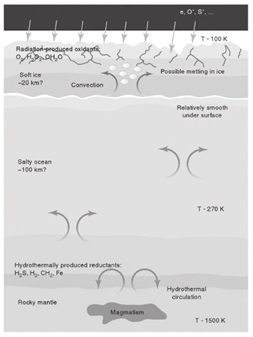
\includegraphics[width=.48\textwidth]{figures/Life/Europasurface}
  \caption{The different process that Europa might have for producing a habitat for life\cite{LifeBeyondEarth}}
  \label{fig:EuropaFromSurfaceToRockcore}
\end{figure}

In conclusion life is very complex to quantify and only a set of guidelines can be set up, derived from the life known to Earth. The guidelines set up give an indication of what to look for, when searching for a habitat or life on another planet, it also points to more precise investigations into what life forms might be found on Europa. It is still difficult to say anything exact of what could be expected to be found on Europa, in form of geology and energy source, but throughout this study it is evident that Europa is a good place the search for life in our solar system. In all Europa ticks many of the right boxes set up for a habitable moon with nutrition and energy to sustain life.

\subsection{Life signal detection in icy oceans}
As it was mentioned in the previous paragraphs, biologists may assume that living organisms on Earth arose from the oceans. Due to this supposition, on icy moons such as Europa or Enceladus, water or ice is the material which has the most potential for life signal detection. Yet, the question might emerge in us, how likely is the habitability of these icy environments? Furthermore how would we search for it?

To get answers to these questions, scientist are using terrestrial analogue environments on Earth to investigate the chemical processes that may occur in the icy oceans. The particular analogue sites, are used to detect and study geological and biological processes which are expected to be on other planets. Such places for example the Cedars, in California or Cabeco de Vide, in Portugal have natural springs that represent extreme metabolic environment as it is assumed to be on Europa. In these places scientists are able to investigate the energy sources produced by water-rock interactions and also the organisms that are using these energy-sources for life.

Only two properties can determine if an object is alive:
metabolism and motion. All living things require the presence of metabolism to remain viable against entropy. However, both metabolism and movement also occur without biological signature.

Presuming that within an extraterrestrial organism the same processes are taking place as under conditions on Earth, metabolism could be effectively examined - according to Isik Kanik physicist.
\cite{astrobio}


As it was mentioned before, metabolism is the set of life-sustaining chemical transformations within the cells of living organisms. Metabolism has three main purposes such as the conversion of food/fuel to energy to run cellular processes, the conversion of food/fuel to building blocks for proteins, lipids, nucleic acids, and some carbohydrates, and the elimination of nitrogenous wastes.
\cite{wiki:metabolism}


So one way to detect existing life is to take a look into how the chemical differences excite metabolisms. However this also requires a challenging method for the biochemists as how to find the marks of these unequaled energy levels.

As it was discussed in the previous paragraphs, the practical way to detect life is to determine what are the essential elements that it requires. These basic elements are: energy, carbon, liquid water, and a few other elements such as nitrogen, sulfur, and phosphorus.
On Earth the vast majority of life forms depend on the solar energy. There are only two methanoged-based ecosystems known, which ultimately gain their productivity from chemical energy.
\cite{10.1371/journal.pbio.0020302}


If we were to find microorganisms in the icy water, how could we decide whether it was the product of a living system or abiotic material? If the environment that we are searching in is similar to the conditions on Earth, then obviously it will be easy for scientists to determine the microorganisms. Although if it differs from what we are used to on Earth, then likely enough the probes, which are specific to our biological circumstances, will not work. In consequence the question is still open for the scientists, how to determine living organisms in the Solar System?

There is a promising approach to decide between the biotic and abiotic materials. It is called the "Lego Principal". The idea is based on the patterns of the molecules of life.

Biotic mechanisms are built on a particular set of organic molecules. These biological organics may have different concentrations of organic compounds, which are chemically very similar to one another. 
Whereas the nonbiological mechanisms are using a wide range of the possible organic molecules and has a smooth distribution as shown in the figure below.
\ref{fig:biological_vs_abiotic}

\begin{figure}[htb]
  \centering
  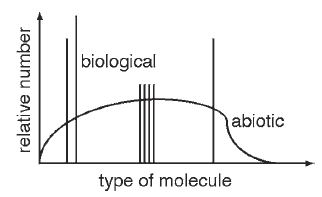
\includegraphics[scale=.9]{figures/BFfig/biological_vs_abiotic}
  \caption{Comparison of biological with abiotic distributions of organic material}
  \label{fig:biological_vs_abiotic}
\end{figure}

This approach may give us a real time result of the relative concentration of molecules. In addition the samples can be easily tested and evaluated. 
It is feasible that the different life forms have various patterns, however scientists might find similarity or even mirror symmetry in the distribution of the concentrations. 

Subsequently, the analysis of the organic compounds might reveal a pattern that is biological despite the fact that it might not be a terrestrial biomolecule which is familiar to humans.


\subsection{Potential habitats on Europa}

The discovery of non-Earth or truly alien life would be a huge step for humanity since it would not only prove that we are not the only ones in the Solar System but also we would get answers to questions like where we came from, what might have been the origin of life on Earth. It would be an enormous and scientifically significant discovery for mankind.

In the previous section we already had an introduction about why to look at Europa. In this paragraph a deeper investigation is carried out about the potential habitats where life forms may appear in the icy ocean.

On Earth, deep on the ocean floor, large colonies of chemosynthetic life is present. These colonies are located around hydrothermal vents and are sustained by chemical energy. 
The same phenomenon might occur on the Jovian satellite Europa because of the tidal forces generated by Jupiter. The ocean-covering ice sheet on Europa is moving, rising and falling tens of meters. This huge energy impact might result in eruptions in the form of hydrothermal vents on the ocean floor, the same way like on Earth.

The presumably life limiting factors such as the radiation and the low temperatures on Europa are precluding the possibility of biological activity on and close to the surface. The plausible habitats for life on Europa are the ice layer, the brine ocean, and the seafloor environment.

However the most likely is the water-ice encounter region since only there can one find  the requisite temperatures and the liquid water.
The figure in the previous chapter reveals these different supposed habitats for life.
\cite{SearchLife}



As it was mentioned previously as well, the oxidation and reduction reactions are the fuel to metabolism. That is, the cycling of oxidants and reductants are necessary to preserve a viable ecosystem.

On the one hand, as a result of the heavy radiation impact on the surface, Europa's exterior layers are strongly oxidizing. On the other hand the ocean and the seafloor sediments are reducing environments. Concerning the composition of the salty water, there are several different hypothesis in the literature. The ocean could be (1) a neutral Na-Mg-SO4-H2O, (2) an alkaline Na-SO4-CO3, or (3) an acidic Na-H-Mg-SO4 system.


The water on Europa might be compositionally and thermally and stratified. Also it should be taken into consideration that depending on the chemical composition, the temperature and the pressure of the brine water may vary. For example for a pure Na-Mg-SO4-H2O system at 1.01 bar is, 238 K, where as the eutectic temperature for a H-Mg-SO4-H2O system at 1.01 bar is 211 K. 


For the reason that presumably there are missive disturbances in the water, scientists assume that this could lead to exsolution of gases and thermal fluxes towards the surface. This phenomenon is called cryovolcanism which may take a part in the cycling of oxidants and heat. Also as it was mentioned before, small hydrothermal vents might serve as refugia in the inhospitable and brusque water.

In the following section we are taking the three ocean layers (ice layer, the brine ocean, and the seafloor environment) on close inspection.

\subsubsection{Life in the ice layers}

Ice could be a possible environment for preserving organics and life forms in the dormant stage. How deep into into the ice could one detect living organisms depend on the many factors such as radiation temperature, pressure, the desiccating power of the environment, solid-state convective flow, and fluid movement along the stress factors. However, if life exists in the external ice layers, it is more likely to find it in the inner regions, yet in the surface because of the destructiveness of the radiation.
Europa is continuously hit by the ionizing particles trapped by the magnetosphere of Jupiter. The table below contains several different organisms and their radiational durability. 
\ref{fig:Organisms_rad_durability}

\begin{figure}[htb]
  \centering
  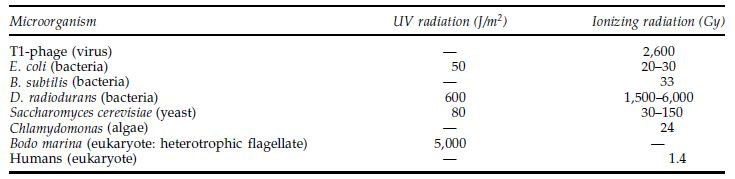
\includegraphics[scale=.8]{figures/BFfig/Organisms_rad_durability}
  \caption{Radiation dose giving around 37 percent survival rate to microorganisms}
  \label{fig:Organisms_rad_durability}
\end{figure}


This radiation is so intense that for a  dose rate of 3–5 Gy/min, for example a bacteria called E. coli and Bacillus would be inactivated within 10 minutes; even the spores of Bacillus, which is hard to destroy, would be inactivated within 40 hours.
Fortunately, as it is known, ice thickness can provide the sufficient protection that is needed to protect the inner layers from the radiation. Most organisms which are not as resistant as for instance D. radiodurans, might survive the radiation below 10 cm.

As it was mentioned before, not only the radiation has an effect on the microbial life but also the temperature. At the surface of the ice, the temperature is approximately 86–132 K which is below the limitation for organisms to survive. The most likely place for habitats to be found is in brine pockets in the bottom of the ice layer.

\subsubsection{The brine ocean and the seafloor environment}

Studies hypothesized that concerning the waters composition, density and temperature, the Europan ocean could be layered.

The temperatures in the seafloor might be substantially warm as a result of the tidal waves dissipation and the internal heat flow from the crust, which could lead to explosive cryovolcanism as mentioned earlier. These places in the bottom of the ocean might be highly desirable for living organisms to grow.
